\chapter{Systems}


\section{Quantum dots}
Strongly confined electrons offer a wide variety of complex and subtle phenomena which pose severe  challenges to existing many-body methods.
Quantum dots in particular, that is, electrons confined in semiconducting heterostructures, exhibit, due to their small size, discrete quantum levels. 
The ground states of, for example, circular dots show similar shell structures and magic numbers as seen for atoms and nuclei.
In this thesis we study quantum dots confined in a nearly two-dimensional thin layer of a semiconductor.
The potential is approximated by a radially symmetric parabolic potential, also called a harmonic-oscillator potential, for which reason they are termed parabolic or circular quantum dots.

Small confined systems, such as quantum dots, have become very popular for experimental 
study. 
Beyond their possible relevance for nanotechnology, they are highly tunable in experiments and introduce level quantization and quantum interference in a controlled way. 
The possibility to manufacture systems with a tailored electronic structure, may improve the electrical or optical properties, a reason why quantum dots are good candidates as components in quantum computers, optimized solar cells, laser technology and medical imaging, to name a few.



\subsection{The Schrödinger equation in spherical coordinates}
Circular quantum dots are said to live in only two dimensions, a consequence of precise manufacturing techniques, making the layers so thin that we can omit the third dimension in our computations.
The quantum dots are, however, not truly two-dimensional and this could lead to an error in the calculated energies.

The harmonic-oscillator potential for two dimensions was encountered in section~\ref{sec:qm:ho2d}, but we will now solve the time-independent Schrödinger equation,
\begin{equation}
-\frac{\hbar^2}{2m}\nabla^2 \psi + \frac{1}{2} m \omega^2 r^2 \psi 
=
E \psi ,
\end{equation}
in spherical coordinates instead of Cartesian.
Assuming the wave function can be separated into two factors depending on radial distance, $r$, and the angle, $\varphi$, we get
\begin{equation}
 \psi   = R(r) Y(\varphi).
\end{equation}
Employing polar coordinates also for the momentum operator, the Schrödinger equation reads,
\begin{equation}
-\frac{\hbar^2}{2m} 
\left(\frac{\partial^2}{\partial r^2} + \frac{1}{r}\frac{\partial}{\partial r} + \frac{1}{r^2}\frac{\partial^2}{\partial \varphi^2}\right)
 R(r) Y(\varphi) + \frac{1}{2} m \omega^2 r^2  R(r) Y(\varphi)
=
E  R(r) Y(\varphi) .
\end{equation}
Dividing by $\hbar^2 R(r) Y(\varphi)$, multiplying with $-2 m r^2$ and reordering terms, we obtain
\begin{equation}
\frac{r^2}{R(r)} 
\frac{\partial^2R(r)}{\partial r^2}
+
\frac{r}{R(r)}
\frac{\partial R(r)}{\partial r} 
-
\frac{2mr^2}{\hbar^2}
\left(\frac{1}{2} m \omega^2 r^2 - E  \right)
=
m_l^2
=
-
\frac{1}{Y(\varphi)}
\frac{\partial^2 Y(\varphi)}{\partial \varphi^2},
\end{equation}
where $m_l$ is our constant of separation.
Thus, we have two equations,
\begin{equation}
\label{eq:qDots:radial}
r^2 \frac{\partial^2R(r)}{\partial r^2}
+
r \frac{\partial R(r)}{\partial r} 
-
\frac{2mr^2}{\hbar^2 }
\left(\frac{1}{2} m \omega^2 r^2 - E  \right)R(r)
=
m_l^2 R(r) ,
\end{equation}
\begin{equation}
\label{eq:qDots:angular}
\frac{\partial^2 Y(\varphi)}{\partial \varphi^2}
=
- m_l^2 Y(\varphi) .
\end{equation}
Equation~\eqref{eq:qDots:angular} is easily recognized as an exponential function,
\begin{equation}
Y(\varphi) = Ke^{i m_l \varphi}, 
\end{equation}
where $K$ is to be determined by normalization,
\begin{equation}
\int_0^{2\pi} Y(\varphi) d\varphi = 1 
\Rightarrow 
Y(\varphi) = \frac{1}{\sqrt{2\pi}} e^{im_l \varphi},
\end{equation}
and rotational invariance determines $m_l$,
\begin{equation}
Y(\varphi) = Y(\varphi + 2\pi) 
\Rightarrow 
e^{im_l 2\pi} = 1
\Rightarrow
m_l = 0,\pm 1,\pm 2, \pm 3, ...   \hspace{2mm}.
\end{equation}
Substituting $R(r) = \rho(r) r^{-\frac{1}{2}}$ eq.~\eqref{eq:qDots:radial} is simplified to
\begin{equation}
\label{eq:qDots:radialEq}
- \frac{\hbar^2}{2m} \frac{\partial^2 \rho(r)}{\partial r^2}
+
\left[
\frac{1}{2} m \omega^2 r^2 
+
\frac{\hbar^2}{2m} \frac{m_l^2 - \frac{1}{4}}{r^2}
\right]\rho(r)
=
E \rho(r) ,
\end{equation}
often named the radial equation.
One should note that this is equivalent to the time-independent Schrödinger equation with an \textit{effective} potential instead,
\begin{equation}
 V_{eff}(r) = V(r) +
\frac{\hbar^2}{2m} \frac{m_l^2 - \frac{1}{4}}{r^2},
\end{equation}
and this strategy can be applied to any system with a spherical symmetric potential.
The full solution after normalization,
\begin{equation}
\int_0^{\infty} |\rho(r) |^2 dr = 1,
\end{equation}
reads
\begin{equation}
\psi(r,\varphi) = \frac{1}{\sqrt{2\pi}} R(r)  e^{im_l \varphi}.
\end{equation}

We will not solve eq.~\eqref{eq:qDots:radialEq} for the one-particle quantum dot here, since it is time consuming and somewhat cumbersome.
Instead we merely state the results and recommend reading the appendix of Lohne's master's thesis~\cite{mplohne} for a full derivation.
The solutions have single-particle energies,
\begin{equation}
\label{eq:qDots:spEnergies}
\epsilon_{n,m_l,m_s} = \left( 1 + |m_l|  + 2 n\right) \omega ,
\end{equation}
with corresponding wave functions,
\begin{equation}
\label{eq:qDots:wavefunc}
\psi_{n,m_l} 
=
\sqrt{\frac{n!}{\pi \left( n + |m_l| \right) !}}
\beta^{\frac{1}{2}\left( 1 + |m_l|\right)}
r^{|m_l|}
e^{-\frac{1}{2}\beta r^2}
L_n^{|m_l|}\left( \beta r^2 \right)
e^{im_l\phi} .
\end{equation}
We have used the Laguerre polynomials, $L_n^{|m_l|}(\beta r^2)$, and also defined
\begin{equation}
\beta = \frac{m \omega}{\hbar}.
\end{equation}
Each spatial wave function from eq.~\eqref{eq:qDots:wavefunc} can have either spin up or spin down.





\section{Implementation}
As a part of this thesis, we have developed a library for running simulations on different types of systems.
The implementation is based primarily on two major types of objects; systems and solvers.
There are two solvers implemented, HF (Hartree-Fock) and CC (Coupled Cluster) to be discussed later, that should work independently of the type of system as long as the system is derived from the `System' base class.
Systems differ, from a computational point of view, only by the value of the one- and two-particle elements, $f_{pq}$ and $\langle pq||rs \rangle$, as well as the number of hole-states, $n_h$, the same as the number of particles, along with the number of unoccupied, virtual, particle-states, $n_p$.
In theory, having an infinite basis, there would be infinitely many particle-states, but in practice it is truncated to a finite set.

\paragraph*{}
`System' has constructs for holding both the one-particle and two-particle interaction matrices, as well as a `Basis' object describing the number of states in addition to how they are stored.
Each unique state is represented with an integer value running from $0$ up to (but not including) the number of states, $n_{tot} = n_p + n_h $.
For the harmonic oscillator basis, `HObasis', states are indexed as in fig.~\ref{fig:qDots:qDotIndex}, first varying $m_l$ in ascending order through all possible values in the lowest-lying shell, holding $|m_l| + 2n = 0$ fixed.
Even states have spin up whereas odd states have spin down, and after one shell is filled indexing starts in the next, $|m_l| + 2n = 1,2,\cdots$ .
It is possible to query the quantum numbers one state, $p$, consists of by calling \mbox{`Basis::stateMap(int p)'}, returning a vector of integer values.
As an example for the harmonic oscillator \mbox{`HObasis::stateMap(10)'} would return a vector
\begin{equation}
\begin{bmatrix}
0 \\
2 \\
0
\end{bmatrix},
\end{equation}
interpreted as $n=0$ and $m_l = 2$ with spin up ($0=\uparrow$ and $1=\downarrow$).
\begin{figure}
\begin{center}
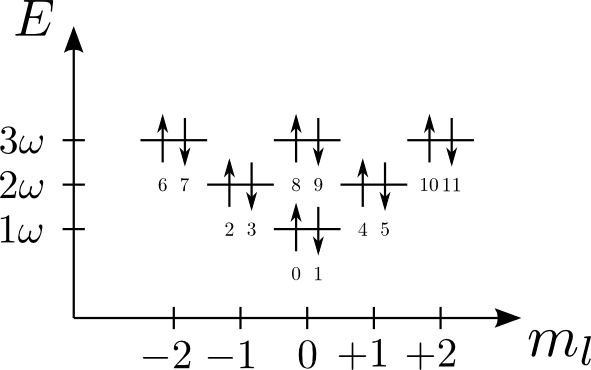
\includegraphics[scale=1.5]{../07-qDots/figs/spektrum.png}
\caption{The indexing sequence used for quantum dots, implemented in `HObasis'.}
\label{fig:qDots:qDotIndex}
\end{center}
\end{figure}



The simplest implementation of a system can be as simple as shown in listing~\ref{lst:qDots:SpecificSystem1}, explained as follows;
\begin{itemize}
\item[Line 1:~] We declare a new subclass of `System'. This provides storage objects for both one-particle and two-particle interactions as well as \textit{getter} methods to these storage objects.
\item[Line 4:~] The most important part in the constructor is to create a sensible `Basis', here using the default basis with 2 electrons (hole-states) and 10 virtual (particle-)states. `fillMatrixElements()' is a method defined in `System' that will fill all storage objects with values from `f\_elem' and `v\_elem' using the size of our basis, stored in `basis'.
\item[Line 12:] `f\_elem' calculates the normal-ordered one-particle element $f_{pq}$, defined in eq.~\eqref{eq:manybody:f_elem}. 
\item[Line 21:] `v\_elem' defines a way to calculate the antisymmetrized two-particle element $\langle pq || rs \rangle $, defined in eq.~\eqref{eq:manybody:v_elem}.
\end{itemize}
\begin{lstlisting}[float,label={lst:qDots:SpecificSystem1},caption={Example on how to implement a specific system by extending the `System' super class.}]
class SpecificSystem1 : public System
{
public:
	SpecificSystem1()
	{
		std::size_t n_elec = 2;
		std::size_t n_virtual = 10;
		this->basis = new Basis(n_elec, n_virtual);
		fillMatrixElements();
	}
	
	virtual double f_elem(std::size_t p, std::size_t q) const
	{
		double h0_pq = //Some expression for h0
		double u_pq = 0;
		for(size_t i = 0; i < basis->get_nH(); i++)
			u_pq += v_elem(p, i, q, i);
		return h0_pq + u_pq;
	}
	
	virtual double v_elem(std::size_t p, std::size_t q, std::size_t r, std::size_t s) const
	{
		double v_pqrs = //Some expression for <pq||rs>
		return v_pqrs;
	}
};
\end{lstlisting}
One should in particular note that these overridden functions are declared virtual. In this way it is possible to create solvers taking a pointer to any `System', still invoking the methods from the correct subclass. 
Listing~\ref{lst:qDots:virtual_p1} illustrates this, using a `System' pointer to access one single-particle element from a specific subclass.
\begin{lstlisting}[float,label={lst:qDots:virtual_p1},caption={A subclass has implemented the function `f\_elem()' returning the element $f_{02}$. The `System' base class has this method declared virtual, resulting in invoking the subclass implementation even when using a super-class pointer.},name={lst:qDots:virtual}]
//anySystem can point to any system,
System * anySystem = new SpecificSystem();
//and still get an element from the correct subclass
double f_02 = anySystem->f_elem(0,2);
\end{lstlisting}

Another way of accessing the same element is to get the storage matrices directly. There are three storage containers for $f_{pq}$; `f\_hh' contains only the part where both $p$ and $q$ are hole-states, `f\_ph' contains only the part where $p$ is a particle-state and $q$ is a hole-state, and `f\_pp' contains only the part with both $p$ and $q$ being particle states.
As an example we recall `SpecificSystem1' having $n_h = 2$ and $n_p = 10$.
If one would like to extract $f_{02}$ one must note that $2$ is the first particle-state, and $0$ is the first hole-state. 
Being symmetric we see how this can be found in the `f\_ph' part,
\begin{equation}
f_{02} = f_{20} = f^{ph}_{00},
\end{equation}
as implemented in listing~\ref{lst:qDots:virtual_p2}.
\begin{lstlisting}[float,label={lst:qDots:virtual_p2},caption={Continuing listing~\ref{lst:qDots:virtual_p1} extracting the same element, $f_{02}$, now through the raw storage matrix for $f$. This example assumes two occupied (hole) states, thus making index $2$ the first ($0$) particle state. With symmetric interaction matrices we expect $f_{ph} = f_{hp}^T$.},name={lst:qDots:virtual}]
mat const * f_hp;
//Get element from raw storage matrix.
f_hp = trans(anySystem->get_f_ph());
f_02 = (*f_ph)(0,0);
\end{lstlisting}

\paragraph*{}
Although the implementation in listing~\ref{lst:qDots:SpecificSystem1} is very simple, counting only 26 lines of code, this would work perfectly for small systems.
For larger systems one would encounter two problems.
Invoking `fillMatrixElements()' will force calculation of all elements every time a `SpecificSystem1' is constructed, a problem discussed later in section~\ref{sec:qDots:TPfile}.
The other problem is that the dimensionality of two-particle interactions scales as the number of virtual states to the fourth power, possibly solved by exploiting symmetries in our Hamiltonian to avoid store a tremendous amount of zero-filled elements.


\subsection{Symmetries in the Hamiltonian}
Two-particle matrix elements $\langle pq||rs \rangle$ can be interpreted as the probability for two particles making a transition from states $r$ and $s$ into $p$ and $q$.
If our Hamiltonian preserves some quantum numbers, this transition is not possible, and thus zero, whenever $pq$ does not preserve the numbers from $rs$.
In the case of quantum dots, we encounter a Hamiltonian that is spherical symmetric, and not spin dependent.
This results in preserving both the angular-momentum quantum number $m (\equiv m_l)$ as well as spin $m_s$.
Defining $M =m^p + m^q, M' = m^r + m^s$ and $M_s = m_s^p + m_s^q, M'_s = m_s^r + m_s^s$, the following holds true,
\begin{equation}
\langle n^p m^p m_s^p; n^q m^q m_s^q || n^r m^r m_s^r; n^s m^s m_s^s \rangle
= 
0
\hspace{3mm}\textrm{if}\hspace{3mm}
M \neq M'
\hspace{3mm}\textrm{or}\hspace{3mm}
M_s \neq M'_s .
\end{equation}

More generally we define a mapping
$(p,q) \leftrightarrow (\lambda,\pi)$
where $\lambda$ is a transition channel, consisting of a specific set of preserved quantum numbers, and a configuration $\pi$ for each possible combination of $(p,q)$ within that channel, such that 
\begin{equation}
\langle \lambda \pi || \lambda' \pi' \rangle = 0
\hspace{3mm}\textrm{if}\hspace{3mm}
\lambda \neq \lambda' .
\end{equation}
This re-indexing allows us to store the interaction elements as a block-diagonal matrix, one block  for each channel $\lambda$, stored as a matrix $\langle \pi || \pi' \rangle_{\lambda}$.
We further split the interaction matrices whether their indices are above ($a,b,c,d$) or below ($i,j,k,l$) the Fermi-level, resulting in six matrices,
\begin{equation}
\label{eq:qDots:split6tpelem}
\begin{split}
\langle ij||kl \rangle& \\
\langle aj||kl \rangle& = -\langle ja||kl \rangle = \langle kl||aj \rangle = -\langle kl||ja \rangle \\
\langle ab||kl \rangle& = \langle kl||ab \rangle \\
\langle aj||cl \rangle& = -\langle aj||lc \rangle = \langle ja||lc \rangle = -\langle ja||cl \rangle\\
\langle ab||cl \rangle& = -\langle ab||lc \rangle = \langle cl||ab \rangle = \langle lc||ab \rangle \\
\langle ab||cd \rangle&  .\\
\end{split}
\end{equation}
Splitting configurations into configurations for hole-hole states, particle-hole states and particle-particle states, yielding the mappings
\begin{equation}
\begin{split}
(i,j) &\leftrightarrow (\lambda, \mu), \\
(a,j) &\leftrightarrow (\lambda, \nu), \\
(a,b) &\leftrightarrow (\lambda, \xi),
\end{split}
\end{equation}
we can use a storage scheme in `System' objects splitting interactions into six parts similarly to eq.~\eqref{eq:qDots:split6tpelem}, exploiting the sparseness to store block-diagonal parts of the six matrices only, 
\begin{equation}
\begin{split}
\langle \mu || \mu' \rangle_{\lambda},& \hspace{5mm}
\langle \nu || \mu \rangle_{\lambda}, \\
\langle \xi || \mu \rangle_{\lambda},& \hspace{5mm}
\langle \nu || \nu \rangle_{\lambda}, \\ 
\langle \xi || \nu \rangle_{\lambda},& \hspace{5mm}
\langle \xi || \xi \rangle_{\lambda} .
\end{split}
\end{equation}

Mappings from states into channels and configurations are managed by the `Basis' class, and one could access these mappings through the eight methods  in listing~\ref{lst:qDots:accessMappings}.
\begin{lstlisting}[float,label={lst:qDots:accessMappings},caption={There are eight different mappings possible to access through the basis object.}]
//Mappings from (pq,lm,dl,de) into lmd and (pi,mu,nu,xi)
get_map_lmdPI_pq();
get_map_lmdMU_lm();
get_map_lmdNU_dl();
get_map_lmdXI_de();

//Reverse mappings 
get_map_pq_lmdPI();
get_map_lm_lmdMU();
get_map_dl_lmdNU();
get_map_de_lmdXI();
\end{lstlisting}
In this context two general states are encoded to one index, $\mathrm{I}$, i.e.
\begin{equation}
\begin{split}
\mathrm{I}(pq) &= p + q \cdot (n_h + n_p) \\
\mathrm{I}(lm) &= l + m \cdot n_h \\
\mathrm{I}(dl) &= d + l \cdot n_p \\
\mathrm{I}(de) &= d + e \cdot n_p,
\end{split}
\end{equation}
where $n_h$ is the number of hole-states, and $n_p$ the number of particle-states.
Returning to our example of `SpecificSystem1' we have $n_h=2, n_p=10$, and trying to access the matrix element $\langle 20||20 \rangle$ we can use either the procedure from listing~\ref{lst:qDots:mapForward}, extracting the raw matrices, or use the `v\_elem' method as in listing~\ref{lst:qDots:mapBackward}.
\begin{lstlisting}[float,label={lst:qDots:mapForward},caption={We try to access the element $\langle 20||20 \rangle$ by mapping the $|20\rangle$ particle-hole state into a channel and a configuration, $|\nu\rangle_{\lambda}$.},name={lst:qDots:map}]
//Create a specific system
SpecificSystem1 sys;

//Get informations about its basis
Basis const * basis = sys.get_basis();
int nH = basis->get_nH(); //hole-states
int nP = basis->get_nP(); //particle-states

//(d,l) = (2,0) is a particle hole configuration.
int d = 2 - nH;
int l = 0;
int dl = d + l * nH;

//Map into a channel and a configuration.
umat const * map = basis->get_map_dl_lmdNU();
int lmd = (*map)(0,dl); //first row contains lambda values.
int nu = (*map)(1,dl); //second row contains configurations.

//Retreive element;
vector<mat> const * phph = sys->get_v_phph();
double elem_20_20 = phph->at(lmd)(nu,nu);
\end{lstlisting}
\begin{lstlisting}[float,label={lst:qDots:mapBackward},caption={Continuing listing~\ref{lst:qDots:mapForward}, accessing the same element again, $\langle \nu || \nu \rangle_{\lambda} = \langle 20||20 \rangle$, now using the reverse mapping, $|\nu\rangle_{\lambda} \rightarrow |20\rangle$.},name={lst:qDots:map}]
//Map back to two states d,l
vector<uvec> const * mapback = basis->get_map_lmdNU_dl();
dl = mapback->at(lmd)(nu);
d = dl % nP + nH;
l = dl / nP;

//this should return the same element
elem_20_20 = sys->v_elem(d,l,d,l);
\end{lstlisting}

\paragraph*{}
The default `Basis' base class will assume only one transition channel, resulting in storing all interaction elements.
For quantum dots we have $M,M_s \leftrightarrow \lambda$, implemented in `HOBasis'.
As an example of the reduced dimensionality, we consider a harmonic oscillator basis with 20 electrons and 400 virtual states.
The largest matrix would be $\langle ab||de \rangle$ with a dimensionality of $400^4$, resulting in $\sim 200$GB of storage!
Exploiting the symmetries and employing an `HOBasis' instead reduces this to $\sim 1.75$GB.
Readers are encouraged to read through this implementation as an example of subclassing `Basis'.



\subsection{Reading elements from file}
\label{sec:qDots:TPfile}
Another time-consuming part is to calculate the matrix elements, which could be performed once and later read from file. 
To create a system read from file, it is convenient to create a subclass of `TPfile', and we take the actual implementation for circular quantum-dots `CQDot' as an example.
There are three methods, shown in listing~\ref{lst:qDots:CQDotMinimumHeader}, which must be overloaded.
\begin{lstlisting}[float,label={lst:qDots:CQDotMinimumHeader},caption={The three most important parts a subclass of `TPfile' would need. The actual implementation of `CQDot' includes some extra methods and private variables.}]
class CQDot : public TPfile
{
public:
  //#1- Constructor
  CQDot(int filledR, int shellsR, double omega = 1.0);
  
  //#2- Calculation of one-particle element f_{pq}
  virtual double f_elem(std::size_t p, std::size_t q) const
  {
    //Part arising from normal ordering
    double u_pq = 0.0;
    for (int i = 0; i < basis->get_nH(); i++)
      u_pq += v_elem(p, i, q, i);
    
	//Part from h0
    ivec3 p_NMMs = basis->stateMap(p);
    int n = pNMMs(0);
    int m = pNMMs(1);
    double h0 = omega * (2 * n + abs(m) + 1);

	//h0 is diagonal
	if (p == q)
      return h0 + u_pq;     
    else
      return u_pq;
  }

protected:
  //#3- A recipe on how to decode tp-element file.
  virtual size_t interp_qNum(char* qNumbers) const;
};
\end{lstlisting}
The constructor takes three arguments; the number of filled shells, the total number of shells and the frequency, $\omega$.

Looking at the constructor's implementation, listing~\ref{lst:qDots:constructor}, we remark how `fillMatrixElements' is no longer called to fill both one- and two-particle elements. 
Instead we read elements $\langle pq||rs \rangle$ from file using `readFileName', and later calculate $f_{pq}$ by invoking 'fillFmatrix'. Both these methods are public, and can therefore be invoked from the main program.
We create a basis, `HOBasis', store the frequency in a private variable, and create a reverse statemap to be used later when reading a file.
This reverse statemap assigns a unique key (unsigned int), constructed from the three quantum numbers, to each state, and it is later possible to get the single index for any state by constructing the same key.
\begin{lstlisting}[float,label={lst:qDots:constructor},caption={Constructor for CQDot.}]
CQDot::CQDot(int filledR, int totalR, double omega)
{
    //Initialize basis and frequency
    basis = new HOBasis(filledR, totalR);
    this->omega = omega;

    //Creating reversed state map, needed when reading file
    int ntot = basis->get_nH() + basis->get_nP();
    for (int state = 0; state < ntot; state++)
    {
    	//Extract quantum numbers n,m,m_s
        ivec3 nmms = basis->stateMap(state);
        unsigned int n = nmms(0);
        int m = nmms(1);
        unsigned int ms = nmms(2);
        
        //Each state has a unique key.
        unsigned int key = n + (m + (ms + hMaxM) * maxM) * maxM;
        revMap[key] = state;
    }
}
\end{lstlisting}

One-particle elements are still calculated through `f\_elem()', implementing the single-particle energies from eq.~\eqref{eq:qDots:spEnergies} combined with a normal-ordered part as in eq.~\eqref{eq:manybody:f_elem}, viz
\begin{equation}
f_{pq} = \delta_{pq} \left(1 + |m| + 2n \right) \omega   + \sum_{i} \langle pi||qi \rangle .
\end{equation}
Depending on $\langle pi||qi \rangle$, one-particle elements are required to be filled first after two-particle elements are read from file, by invoking `fillFmatrix'.

Two-particle elements are read through the method `readFileName', redirecting to `readFileStream' in listing~\ref{lst:qDots:readFileStream}.
The file-reading itself is already implemented in the base class, and we expect elements on file to be for $\omega=1$, such that we need only to scale $\omega$ after reading.
Invoking `TPfile::readFileStream' will force the base-class implementation to be run even though these functions are declared as virtual.
The last steps are to scale elements\footnote{Only standard interaction can be scaled by $\sqrt{\omega}$, forcing us to create another file-reading routine `readEffFileStream' (and `readEffFileName') for effective interactions.} by $\sqrt{\omega}$ and fill the single-particle elements.
\begin{lstlisting}[float,label={lst:qDots:readFileStream},caption={How to read tp-elements for CQDot.}]
void CQDot::readFileStream(std::ifstream &file)
{
    //First read file as done in super class.
    TPfile::readFileStream(file);
    //Then scale by sqrt(omega)
    size_t dimLMD = basis->dim_lmd_2p();
    for (size_t lmd = 0; lmd < dimLMD; lmd++)
    {
        v_hhhh.at(lmd) = sqrt(omega) * v_hhhh.at(lmd);
        v_phhh.at(lmd) = sqrt(omega) * v_phhh.at(lmd);
        v_pphh.at(lmd) = sqrt(omega) * v_pphh.at(lmd);
        v_phph.at(lmd) = sqrt(omega) * v_phph.at(lmd);
        v_ppph.at(lmd) = sqrt(omega) * v_ppph.at(lmd);
        v_pppp.at(lmd) = sqrt(omega) * v_pppp.at(lmd);
    }
    //Fill one-particle elements.
    fillFmatrix();
}
\end{lstlisting}

In order to successfully read elements from file the base class needs some information about the file structure, found through the sub-class implementation of `interp\_qNum'.
A basic file format is expected to be binary with the content,
\begin{verbatim}
p q r s <pq||rs> p' q' r' s' <p'q'||r's'> ... ,
\end{verbatim}
p is a number of bytes, $n_{b}$, needed to specify the state $p$, q is $n_b$ bytes necessary to specify $q$, and so on until the element itself $\langle pq||rs \rangle$ stored as a `double'. 
The implementation for quantum dots may serve as an example.
Here $n,m$ and $m_s$ are coded as an unsigned short, a short and a char. 
This is repeated for all four states an element consists of, followed by the element itself,
\begin{equation}
\underbrace{
\overbrace{n^p}^\text{ushort (2B)} 
\overbrace{m^p}^\text{short (2B)}
\overbrace{m_s^p}^\text{char (1B)}
}_\text{numBytes (5B)}
\underbrace{n^q m^q m_s^q}_\text{(5B)}
\underbrace{n^r\hspace{2mm}m^r\hspace{2mm}m_s^r\hspace{2mm}}_\text{(5B)}
\underbrace{n^s\hspace{2mm}m^s\hspace{2mm}m_s^s\hspace{2mm}}_\text{(5B)}
\underbrace{\langle pq||rs \rangle}_\text{double (8B)} .
\end{equation}
On most platforms this would require 5 bytes for each state, and 8 bytes for the element, as noted in parentheses.
In order to know how many bytes are expected to describe each state, `interp\_qNum(NULL)' is queried.
Once those bytes are read from file they are sent to the same method as a char array, and expected return is a single integer indexing the correct state.
For `CQDot', implementation in listing~\ref{lst:qDots:interp_qNum}, the char array is split into an unsigned short, short and a char, and correct state is found using the reverse state map that was initialized in the constructor.
\begin{lstlisting}[float,label={lst:qDots:interp_qNum},caption={Implementation of `interp\_qNum' in `CQDot'.}]
size_t CQDot::interp_qNum(char* qNumbers) const
{
    //Quantum numbers n, m, m_s read from file.
    unsigned short n;
    short m;
    char ms;
    
    //Single indexed state
    size_t state;

    //The number of bytes for each state
    if (qNumbers == NULL)
        return sizeof (n) + sizeof (m) + sizeof (ms);

    //Split qNumbers!
    size_t siz_n = sizeof (n);
    memcpy(&n, qNumbers, siz_n);
    size_t siz_m = sizeof (m);
    memcpy(&m, qNumbers + siz_n, siz_m);
    size_t siz_ms = sizeof (ms);
    memcpy(&ms, qNumbers + siz_n + siz_m, siz_ms);

    //Encode spin
    if (ms == -1) 
        ms = 1; //down
    else if (ms == +1)
        ms = 0; //up
    
    //unique key for any state
    unsigned int key = n + (m + (ms + hMaxM) * maxM) * maxM;
    //revMap is a std::map filled in the constructor
    const map<unsigned int, unsigned int>::const_iterator found = revMap.find(key);
    
    if (found == revMap.end())
        state = maxM;  //A state outside the current basis
    else
        state = found->second; //State found in current basis

    return state;
}
\end{lstlisting}


A complete file can be read from file in a simple way, as listing~\ref{lst:qDots:readElem} shows, reading one element at a time, adding a  simple loop to read all elements in a file.
\begin{lstlisting}[float,label={lst:qDots:readElem},caption={How to read two-particle elements from file.}]
void TPfile::readFileStream(std::ifstream &file)
{
  //Number of bytes to read for each state.
  size_t qNumWidth = interp_qNum(NULL);
  char * qNumP = new char[qNumWidth];
  char * qNumQ = new char[qNumWidth];
  char * qNumR = new char[qNumWidth];
  char * qNumS = new char[qNumWidth];

  //Allocate memory for tp-elements.
  //......

  while (true)
  {
    //Read one `line' from file
    double element = 0;
    file.read(qNumP, sizeof (char) * qNumWidth);
    file.read(qNumQ, sizeof (char) * qNumWidth);
    file.read(qNumR, sizeof (char) * qNumWidth);
    file.read(qNumS, sizeof (char) * qNumWidth);
    file.read((char*) &element, sizeof (double));
    if (file.eof())
      break;  //End of file?

	//Find the index
    size_t p = interp_qNum(qNumP);
    size_t q = interp_qNum(qNumQ);
    size_t r = interp_qNum(qNumR);
    size_t s = interp_qNum(qNumS);

    //Store all antisymmetric possibilities 
    storePQRS(p, q, r, s, element);
    storePQRS(p, q, s, r, -element);
    storePQRS(q, p, s, r, element);
    storePQRS(q, p, r, s, -element);
  }

  //Free the four char arrays
  //......
}
\end{lstlisting}
The functionality to read files is already implemented in the two methods `readFileName' and `readFileStream'.






\section{Other systems}
Other systems may equally well be implemented, and should be compatible with the different solvers as long as they extend the `System' and `Basis' base classes properly.
As an example we have implemented a simple class, `Atoms', outlined in listings~\ref{lst:qDots:atoms_p1} and~\ref{lst:qDots:atoms_p2}, that include the 8 lowest-lying s-states\footnote{Atomic orbitals are distinguished by their angular momentum quantum number $l$. If $l=0$ the state is said to be \textbf{s}harp, an `s-state'. Continuing, for $l=1,2,3$, we have \textbf{p}rinciple, \textbf{d}iffuse and \textbf{f}undamental.} of atomic orbitals.
The single-particle energies are found in the Bohr-model to be
\begin{equation}
E_n = \frac{Z^2}{2n^2}, \hspace{4mm}\textrm{(in atomic units)},
\end{equation}
and the two-particle correlation elements are found by integrating the Coloumb energies for the atomic orbitals, either calculated analytically by hand or computer algebra software, or by numerical integration.
\begin{lstlisting}[float,label={lst:qDots:atoms_p1},caption={Simple implementation for the first sharp atomic orbitals. Continued in listing~\ref{lst:qDots:atoms_p2}.},name={lst:qDots:atoms}]
class Atoms : public System
{
public:
  /** numElec is 2 for helium, 4 for beryllium */
  Atoms(int numElec = 2)
  {
    //Charge from nucleus defaults to number of electrons
    Z = numElec;
    //There are only 8 states implemented
    basis = new Basis(numElec, 8 - numElec);
    //Fill matrices
    fillMatrixElements();
  }

  virtual double f_elem(std::size_t p, std::size_t q) const
  {
    //Normal-ordered part
    double u_pq = 0;
    for (int i = 0; i < basis->get_nH(); i++)
        u_pq += v_elem(p, i, q, i);
	//single-particle energies
    int n = p / 2 + 1;	 //n is the energy level
	double h0 = -pow((double) Z, 2) / (2 * n * n);
	//h0 is diagonal
    if (p == q)
      return h0 + u_pq;
    else
      return u_pq;
  }
\end{lstlisting}
\begin{lstlisting}[float,label={lst:qDots:atoms_p2},caption={Continuation of listing~\ref{lst:qDots:atoms_p1}.},name={lst:qDots:atoms}]
  virtual double v_elem(
    std::size_t p, std::size_t q,
    std::size_t r, std::size_t s) const
  {
    //Get spin of particles
    bool pUP = p % 2 == 0;
	//... same for q,r and s ...

    //Map p,q,r,s to n quantum number
    int n_p = p / 2 + 1;
    //... same for q,r and s ...

    //First term of element
    double term1 = 0;
    if (pUP == rUP && qUP == sUP)
        term1 = spatial_integral(n_p, n_q, n_r, n_s);
    //Second term
    double term2 = 0;
    if (pUP == sUP && qUP == rUP)
        term2 = spatial_integral(n_p, n_q, n_s, n_r);
	
    return term1 - term2;
  }

  /** The spatial integral of correlation energies can be
  /*  found analytically (and tabulated) using Mathematica
  /*  or Maple. Also possible to find through numerical
  /*  integration. (four lowest lying orbitals only) */
  double spatial_integral(int n_p, int n_q, int n_r, int n_s) const;
            
private:
  /** The total charge in the nucleus */
  double Z ;
};
\end{lstlisting}


\paragraph{}
If we were to extend the Harmonic Oscillator basis to three dimension, we would have a basis often used in nuclear physics. 
In that case, one would need one additional quantum numbers for the orbitals, as well as quantum numbers describing different types of particles.
Although not done in this thesis, it should, in the author's opinion, not be too complicated.
However, nuclear calculations often require a larger dimensionality, and further simplifications, known as jj scheme, exist.

\paragraph{}
The hierarchy of implemented classes is shown in fig.~\ref{fig:qDots:classTree}, where `CQDot', `TPfile' and `Atoms' are already discussed.
`HFsys' is used to obtain a Hartree-Fock transformed basis, as discussed in the next chapter, copying the basis object and transforming the elements from any arbitrary system.
\begin{figure}
\begin{center}
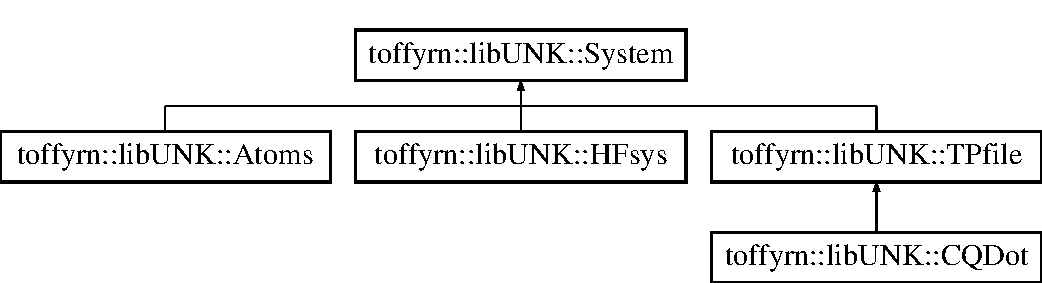
\includegraphics[scale=0.8]{../07-qDots/figs/classTree.pdf}
\caption{Hierarchy of implemented `System' subclasses. `CQDot' is our implementation for circular quantum dots, gaining simplicity by extending the file-reading methods from `TPfile'. `Atoms' defines a simple system including a basis of a few atomic orbitals. The last class, `HFsys', can obtain a Hartree-Fock transformed basis from any other system, as discussed in the next chapter.}
\label{fig:qDots:classTree}
\end{center}
\end{figure}




